\documentclass{evolang11}
\usepackage{graphicx}
\usepackage{url}
\usepackage{pbox}
\usepackage[caption=false]{subfig}
\usepackage{wrapfig}
\usepackage{enumitem}
\setlist{nosep}
\usepackage{sidecap}



\begin{document}

\title{FREQUENCY-DEPENDENT REGULARIZATION IN ITERATED LEARNING}

\author{ANONYMOUS AUTHOR 1}

\address{University Department, University Name \\ City, Country\\email@university}

\maketitle

\abstracts{Binomial expressions are more \emph{regularized}---their ordering preferences (e.g. ``bread and butter'' vs.\ ``butter and bread'') are more extreme---the higher their frequency. Although standard iterated-learning models of language evolution can encode overall regularization biases, the stationary distributions in these standard models do not exhibit a relationship between expression frequency and regularization.  Here we show that introducing a frequency-\emph{independent} regularization bias into the data-generation stage of a 2-Alternative Iterated Learning Model yields frequency-\emph{dependent} regularization in the stationary distribution.  We also show that this model accounts for the distribution of binomial ordering preferences seen in corpus data.}


\section{Introduction}
Languages are shaped both by the cognitive architectures of individual speakers and by the process of cultural transmission that acts across generations. In this paper we ask how these two factors jointly contribute to a key dichotomy in language structure: the trade-off between broadly-applicable compositional knowledge and knowledge of item-specific idiosyncrasies. Specifically, we take up the case of frequency dependence in \emph{regularization}---the extremity of a preference for a given form among multiple alternatives. Although regularization is a well-attested phenomenon in statistical learning, \emph{frequency-dependent} regularization is not. Here we demonstrate that frequency dependence of regularization can arise as an emergent property of a frequency-\emph{independent} regularization bias in language production, combined with the bottleneck effect of cultural transmission.

Item-specific idiosyncrasies (i.e\ exceptions to the rules) are well known to be frequency-dependent. For example, more frequent verbs are more likely to have irregular conjugations \cite{Lieberman:2007bl}.
%\cite{KIRBY:2001wt} has demonstrated that this pattern can emerge as a result of competing pressures during cultural transmission: a ``learning bottleneck'' (i.e.\ a restriction on the number of utterances heard per generation) favors compositionality, which allows form-meaning mappings to be induced in the absence of substantial direct experience with a given item. In contrast, a ``production bottleneck'' favors short utterances, which is at odds with compositionality (under the reasonable assumption that the compositional units each consist of their own linguistic material, and therefore compositional forms are required to be longer on average than non-compositional forms). For less frequent items, the learning bottleneck is stronger, favoring regular/compositional forms. For more frequent items, the learning bottleneck is weaker, and shorter, irregular forms can prevail.
More recently, \citeA{Morgan:2015to} have demonstrated a different type of frequency-dependent idiosyncrasy at the level of multi-word phrases, specifically \emph{binomial expressions} of the form ``X and Y'' \cite{Cooper:1975uz,Benor:2006gv}. Word order preferences for these expressions are gradient; for example, ``radio and television'' is preferred to ``television and radio'' in a 63 to 37 ratio, while ``bread and butter'' is preferred to ``butter and bread'' 99 to 1 \cite{Lin:2012te}. These ordering preferences are partially determined by productive, violable constraints, e.g.\ a constraint to put shorter words before longer words. But these expressions are also subject to learned item-specific idiosyncrasies, e.g. despite a generally strong constraint to put men before women, ``ladies and gentlemen'' is preferred over ``gentlemen and ladies''. In addition to the possibility of the complete reversal of compositional preferences, item-specific idiosyncrasies can also be gradient, e.g.\ a binomial whose compositional preference predicts a 60/40 distribution might instead be used in a 90/10 ratio. 
%
\citeA{Morgan:2015to} showed that, as is the case  with irregular verbs, the distribution of idiosyncrasies in binomial ordering preference is frequency-dependent: more frequent binomial expressions deviate more from compositional preferences.  In particular, more frequent binomials are more strongly regularized.
%\footnote{Following previous evolutionary linguistics literature, we define \emph{regularization} as reduction in entropy of a distribution, i.e.\ reduction in variation. We note that this is different from the notion of ``regular'' items as those that conform to compositional rules.}
%\footnote{In other evolutionary linguistics literature, our notion of \emph{polarization} is often referred to as \emph{regularization}. We avoid this term because it has the potential for contradictory meanings in the domain of binomial expressions: In one sense, regularization refers to distributions that have lower entropy or \textbf{less variation}, such as expressions that occur more consistently in a given order. In another sense, regular items are those that conform to compositional rules, which in the case of binomial expressions tends to mean exhibiting \textbf{more variation}. To avoid confusion, we use the terms \emph{polarization} and \emph{reducing variability} to refer to the entropy of distributions and the terms \emph{compositional} versus \emph{idiosyncratic} to refer to whether an item is rule-following.}

Regularization is a well-established phenomenon in statistical learning. In a variety of tasks, both linguistic and non-linguistic, in which participants learn and reproduce probability distributions over alternates, both children and adults tend to regularize their productions \cite{HudsonKam:2005we,Reali:2009dp,FERDINAND:2014tk}. For example, \citeA{Reali:2009dp} found that when exposed to two labels for a novel object, subjects reproduced the more frequent label \emph{even more frequently} than that label was seen in training. Although this tendency was weak, they demonstrated that even such a small bias towards regularization can have significant long-term impacts, as the bias acts across successive generations to shape language over time.  \citeA{Bickerton:1981ve}, \citeA{HudsonKam:2005we}, and others have argued that children's tendency to regularize is an important mechanism of language change, e.g.\ for forming more consistent languages out of pidgins.

% However, to the best of our knowledge, there has been no previous demonstration of regularization being dependent upon the frequency of an item (not to be confused with the frequency of the forms used to label the item)---e.g. in Reali and Griffiths's experiments, regularization was not dependent upon the frequency of occurrence of the novel object---nor is it immediately predicted by any existing theories. 
However, standard iterated-learning theories of language evolution do not, in general, lead to frequency-dependent regularization.  Thus Morgan and Levy's finding is unexpected, and poses a challenge to models of language evolution. In this paper, we review the key data (Section~\ref{sec:dataset}) and show that standard iterated-learning models fail to account for frequency-dependent regularization (Section~\ref{sec:regul-freq-indep}). We then show that frequency-dependent regularization emerges when the data-generation stage of a standard iterated learning model is augmented with a frequency-independent regularization bias, and that this augmented model accounts for the empirical distribution of binomial ordering preferences (Section~\ref{sec:emerg-freq-depend}). Section~\ref{sec:conclusion} concludes.

\section{Dataset}
\label{sec:dataset}
%
We take advantage of a uniquely appropriate real-world data set: \citeA{Morgan:2015to}'s corpus of 594 binomial expression types hand-annotated for a range of semantic, phonological, and lexical constraints known to affect binomial ordering preferences, and with frequencies of each ordering extracted from the Google Books corpus \cite{Lin:2012te}. Morgan and Levy also reported a model estimating the quantitative compositional ordering preference for each binomial expression, as expected on the basis of the above constraints (independent of actual occurrence frequencies). The dataset and model thus give us three key measures for these expressions:
%
\begin{itemize}
\item The \emph{overall (unordered) frequency} of an expression: freq(``X and Y'')$+$freq(``Y and X'')
\item The \emph{observed preference} for occurrence in a given order, expressed as a number between 0 and 1: freq(``X and Y'')$/$(freq(``X and Y'')$+$freq(``Y and X''))
\item The \emph{compositional preference} for occurrence in a given order, expressed as a number between 0 and 1, given by Morgan and Levy's model.
\end{itemize}
%
Observed preferences are multimodally distributed, with modes at the extremes as well as around 0.5 (Fig.\ \ref{fig:corpus}). Crucially, this pattern is not predicted by compositional preferences, which predict only a single mode (Fig.\ \ref{fig:logistic}). This pattern reflects the key generalization to be accounted for in the present paper: that expressions with higher overall frequency diverge most from compositional preferences, and are more regularized (Fig.\ \ref{fig:extremity}).  

% We ask what combination of individual cognitive biases and properties of cultural transmission predict the patterns seen in Figs.\ \ref{fig:corpus} and \ref{fig:extremity}. We will see that a standard 2-Alternative Iterated Learning Model does not correctly predict these patterns, but an augmented model with an explicit regularization bias does.

 \begin{figure}[t]
\begin{center}
	\subfloat[]{
	        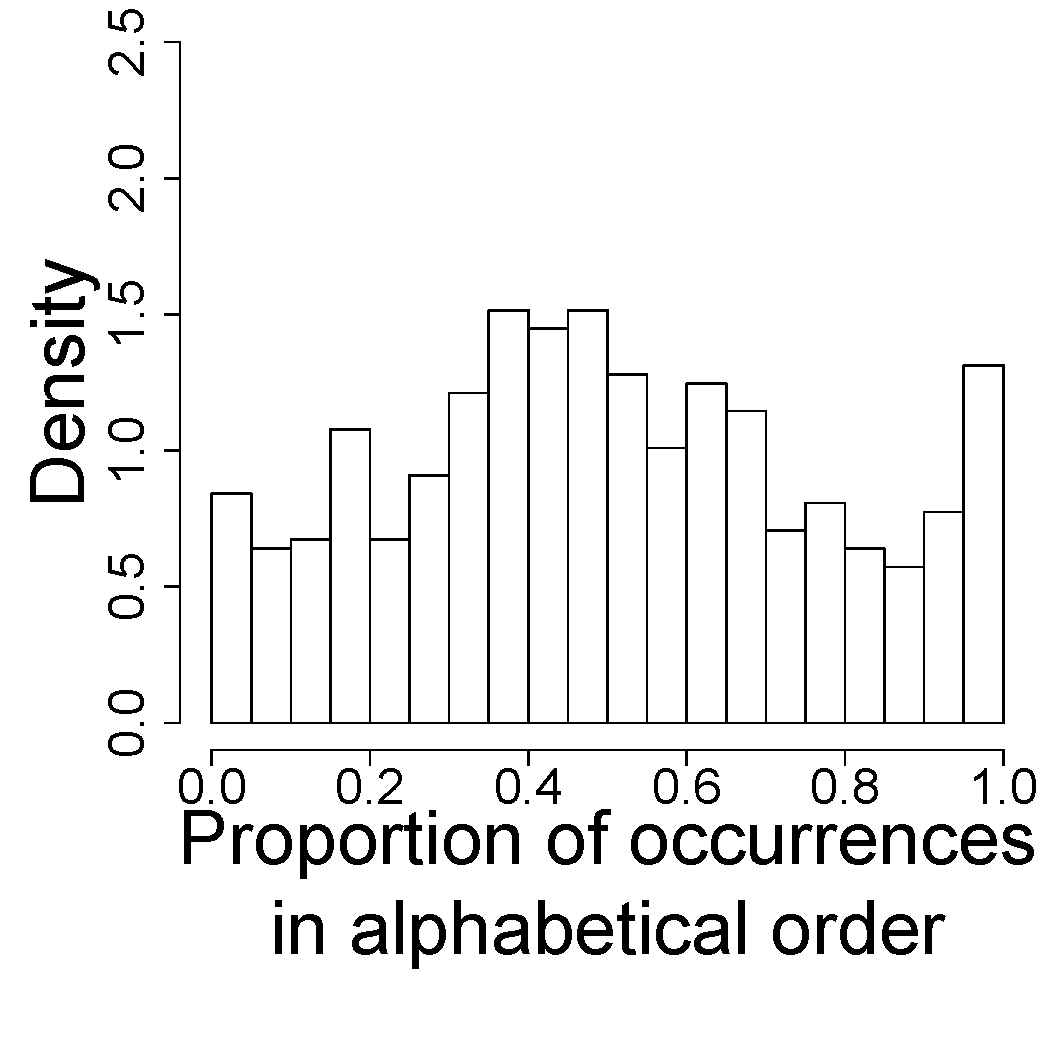
\includegraphics[scale=.2]{corpus-hist.pdf}\label{fig:corpus}
	}
	\subfloat[]{
	        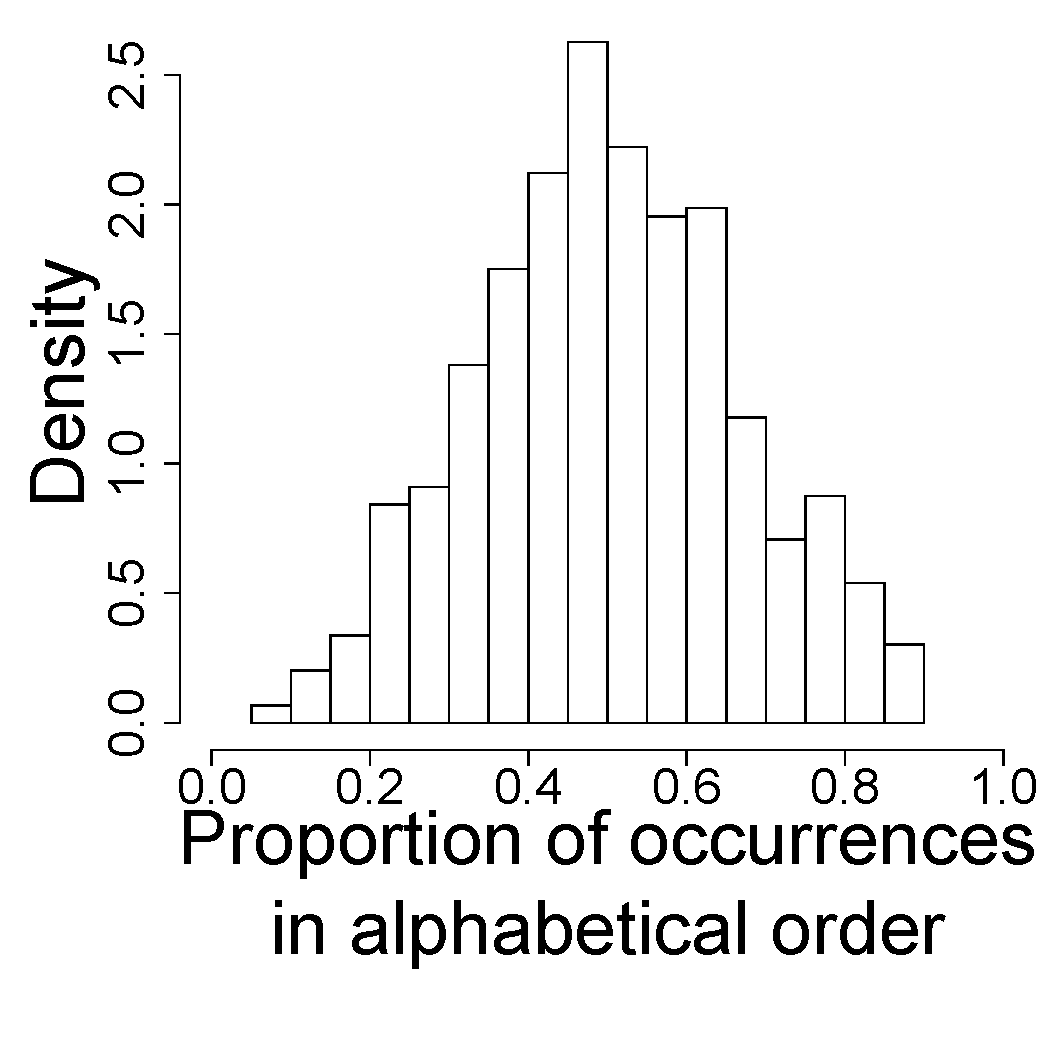
\includegraphics[scale=.2]{logistic-hist.pdf}\label{fig:logistic}
	}
	\subfloat[]{
	        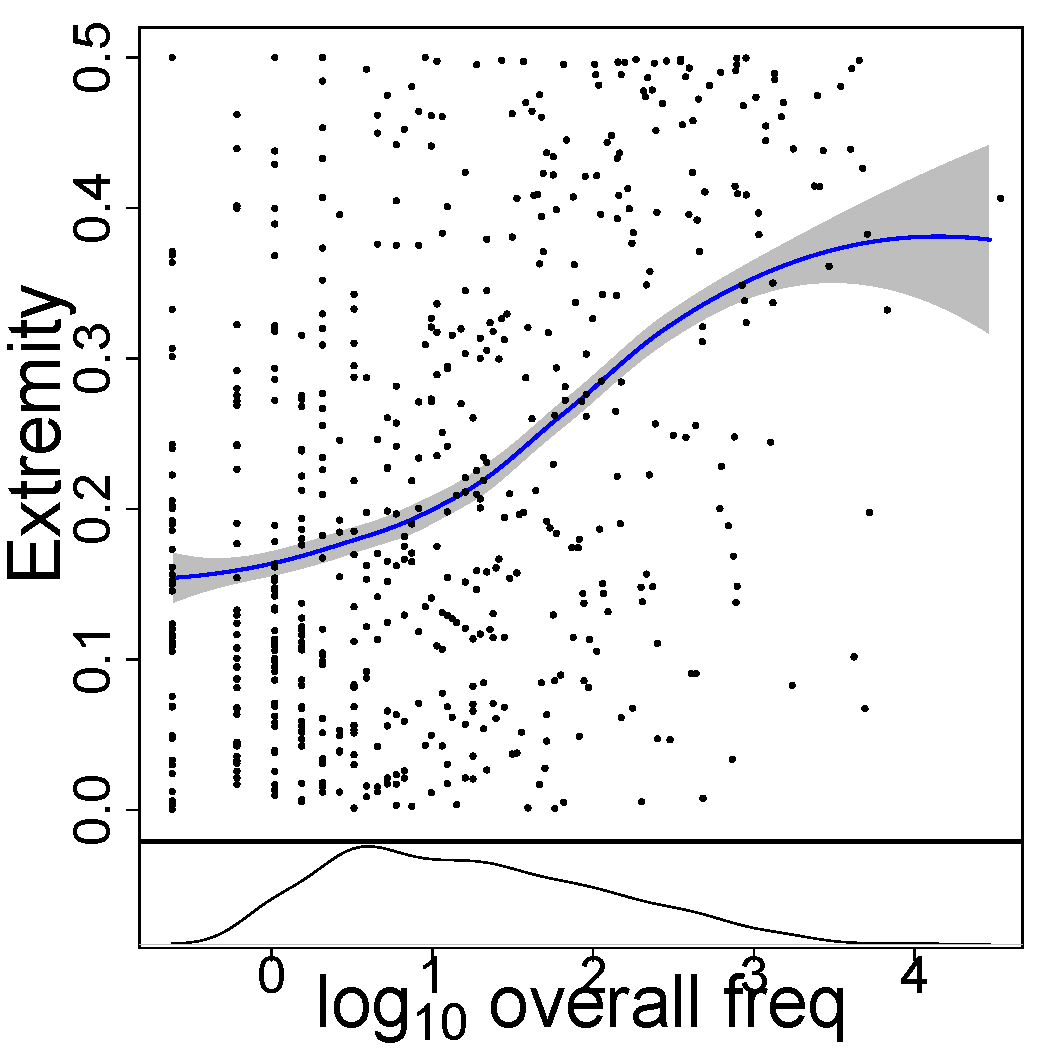
\includegraphics[scale=.2]{Fig1c/extremity-roger.pdf}\label{fig:extremity}
	}

\end{center}
\caption{\footnotesize Results from Morgan and Levy (2015).  (a) Histogram of binomial types' observed preferences. (b) Histogram of binomial types' compositional preferences. (c) We define an expression's \emph{extremity} as the absolute difference between its observed preference and 0.5. More frequent expressions have more extreme/regularized preferences; see Morgan \& Levy (2015) for alternative ways to quantify extremity that yield similar conclusions. Lower panel shows density of overall frequency counts (scaled as described in Section \ref{corpus}). The distribution is non-Zipfian because the corpus is restricted to binomial types with at least 1000 occurrences in the Google Books corpus to ensure accurate observed preference estimates.}
\end{figure}



\section{Regularization is Frequency-Independent in Standard Iterated Learning}
\label{sec:regul-freq-indep}
%
We use 2-alternative iterated learning \cite{Reali:2009dp,SMITH:2009uw} to simulate the evolution of binomial expressions over generations of speakers.
%Specifically, a learner in a given generation has some hypothesis $h$ which they use to stochastically produce data $d$. A learner in the next generation then learns a new hypothesis using Bayes rule, which defines a probability distribution over hypotheses:
%\begin{equation}
%P(h|d) = \frac{P(d|h)P(h)}{P(d)}\label{eq:bayes}
%\end{equation}
%The learner can choose a hypothesis from this distribution by various means. In particular, methods that are often studied are sampling or taking the \emph{maximum a posteriori (MAP)} estimate.
 A learner hears $N$ tokens of a binomial expression, with $x_1$ of them in a given order---we use alphabetical order as a neutral reference order---and then infers a hypothesis $\theta_1 \in [0,1]$ which is the proportion of time a binomial should be produced in alphabetical order. The learner then generates new data using $\theta_1$.
 
The prior probability $P(\theta_1)$ of a binomial being preferred in a given order can be expressed using the beta distribution. We can treat the compositional preference as a form of prior knowledge of ordering preferences for a binomial. To incorporate this prior knowledge, we use a parameterization of the beta distribution with a parameter $\mu$ that determines the mean of draws and a concentration parameter $\nu$ that determines how tightly clustered around the mean those draws are. ($\nu$ can also be thought of as reflecting how confident in the prior we are, e.g. $\nu=10$ would indicate confidence equivalent to having seen ten instances of a given binomial expression type before.) Under this parameterization,
\begin{equation}
P(\theta_1) = \frac{\theta_1^{\mu\nu-1}(1-\theta_1)^{(1-\mu)\nu-1}}{\mathrm{B}(\mu\nu,(1-\mu)\nu)}
\end{equation}
where $\mathrm{B}$ is the beta function. Because $\mu$ represents compositional ordering preferences, it varies for each binomial, and is set according to Morgan and Levy's model. All learners are assumed to have the same $\mu$ value for a given binomial. $\nu$ is constant for all binomial expressions for all learners, and is a free parameter. Given $\theta_1$, data is generated binomially:
\begin{equation}
P(x_1|\theta_1) = \binom{N}{x_1}\theta_1^{x_1}(1-\theta_1)^{N-x_1}\label{eq:binomial}
\end{equation}

%\footnote{This is equivalent to a beta distribution with the more familiar pseudocount parameterization where $\alpha_1=\mu\nu$ and $\alpha_2=(1-\mu)\nu$.}

We define a chain of learners under this model by initializing a single learner with some hypothesis. This first generation produces $N$ utterances according to the distribution defined in Eq.\ \ref{eq:binomial}. The learner in the next generation applies Bayes rule and chooses a hypothesis from the resulting posterior distribution over hypotheses. This process continues iteratively.

\citeA{Reali:2009dp} have demonstrated that regularization occurs in iterated learning models with sparse priors (i.e. those that favor hypothesis close to 0 and 1); given our parameterization of the beta distribution, these are hypothesis with $\nu<2$. However, this regularization is not dependent on the expression's overall frequency. We demonstrate this by modeling chains of learners with different values of $N$. We model a single binomial expression with prior probability $\mu=0.6$. We explore different values of $\nu$, specifically $\nu=1$ (a sparse prior) and $\nu=10$ (a dense prior). We explore values of $N=10,100,200,500$. For each combination of $\nu$ and $N$, we approximate the distribution over expression preferences by running 500 chains of learners for 500 generations each and taking the hypothesis of the final generation in each chain. (For all chains in all simulations in this paper, we initialize $\theta_1=0.5$ and use MAP estimation to choose $\theta_1$ in each new generation. Results are qualitatively similar under posterior sampling.)  Regularization in the resulting distributions does not depend on $N$. (Fig.\ \ref{fig:R11}; the apparent exception---$N=500, \nu=1$---is due to not running the simulation long enough for these chains to converge to their stationary distribution. Higher values of $N$ lead to slower convergence.) In other words, the number of times an expression is seen in each generation does not affect its ultimate degree of regularization.


\begin{figure}[t]
 \setlength\tabcolsep{1pt}
\begin{center}
  \begin{tabular}{lcc}
 & $\nu = 1$ &  $\nu = 10$
  \\
  $N=10$ & \pbox[c]{\textwidth}{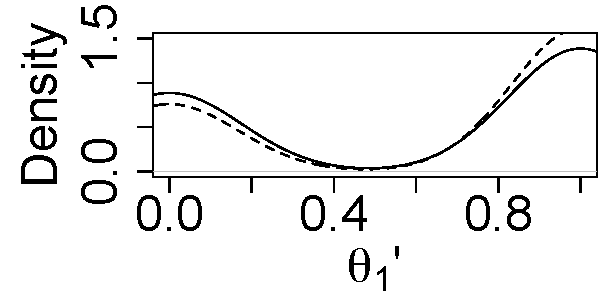
\includegraphics[scale=.3]{sims-R-1-1.pdf}}
%  & \pbox[c]{\textwidth}{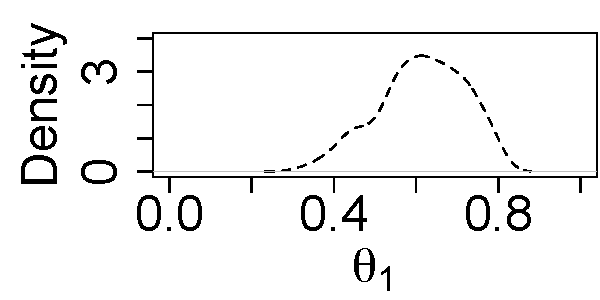
\includegraphics[scale=.3]{sims-10-1.pdf}}
  & \pbox[c]{\textwidth}{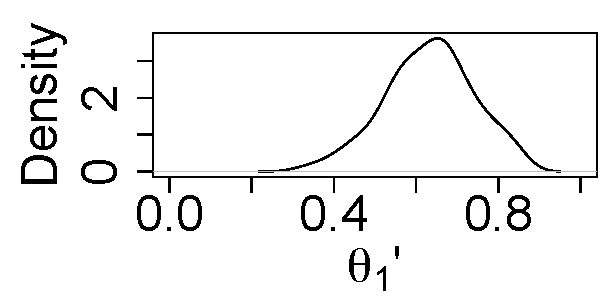
\includegraphics[scale=.3]{sims-R-10-1.pdf}}
\\
  $N=100$ & \pbox[c]{\textwidth}{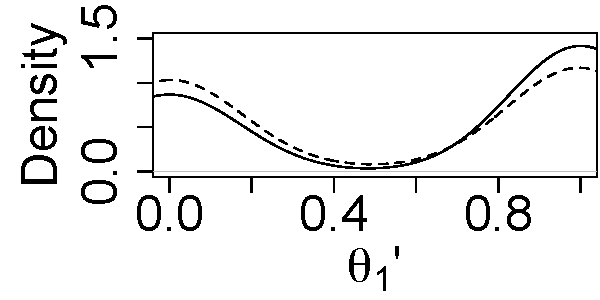
\includegraphics[scale=.3]{sims-R-1-2.pdf}}
%    & \pbox[c]{\textwidth}{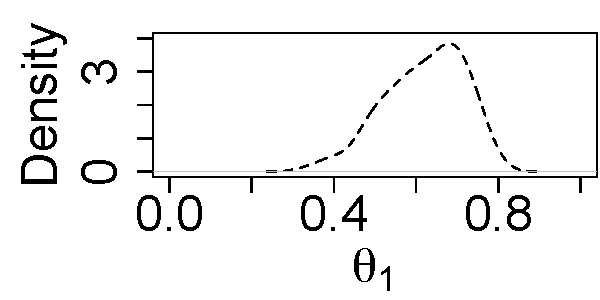
\includegraphics[scale=.3]{sims-10-2.pdf}}
  & \pbox[c]{\textwidth}{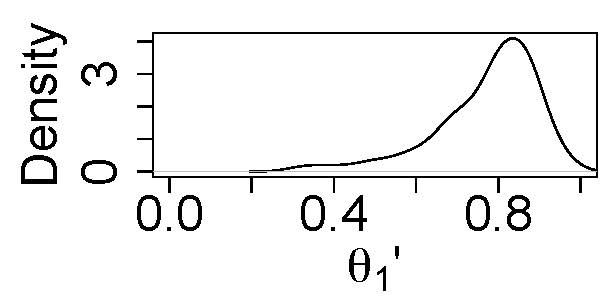
\includegraphics[scale=.3]{sims-R-10-2.pdf}}
\\
  $N=200$ & \pbox[c]{\textwidth}{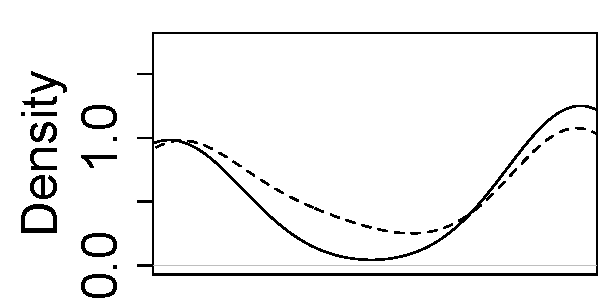
\includegraphics[scale=.3]{sims-R-1-3.pdf}}
%    & \pbox[c]{\textwidth}{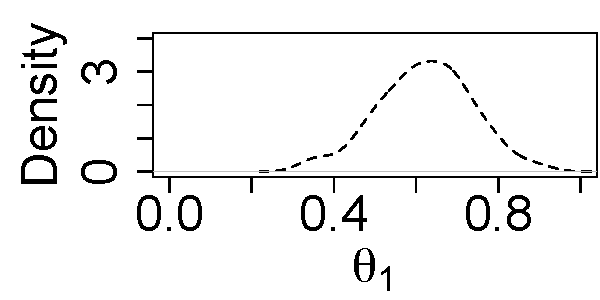
\includegraphics[scale=.3]{sims-10-3.pdf}}
  & \pbox[c]{\textwidth}{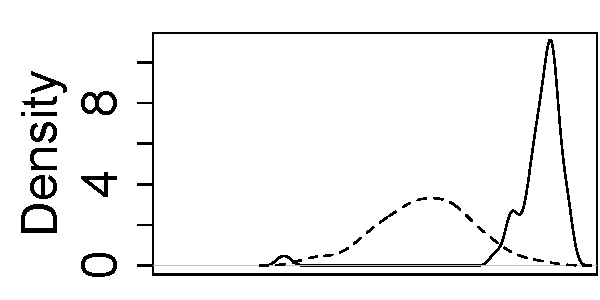
\includegraphics[scale=.3]{sims-R-10-3.pdf}}
\\
  $N=500$ & \pbox[c]{\textwidth}{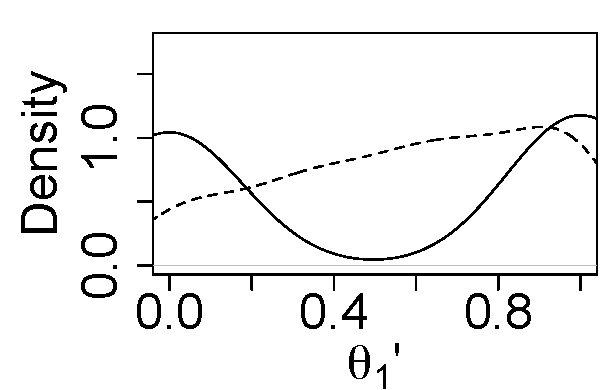
\includegraphics[scale=.3]{sims-R-1-4.pdf}}
%    & \pbox[c]{\textwidth}{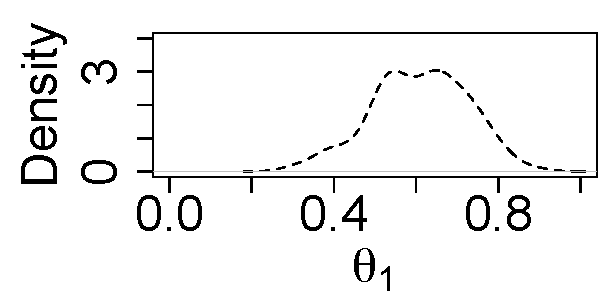
\includegraphics[scale=.3]{sims-10-4.pdf}}
  & \pbox[c]{\textwidth}{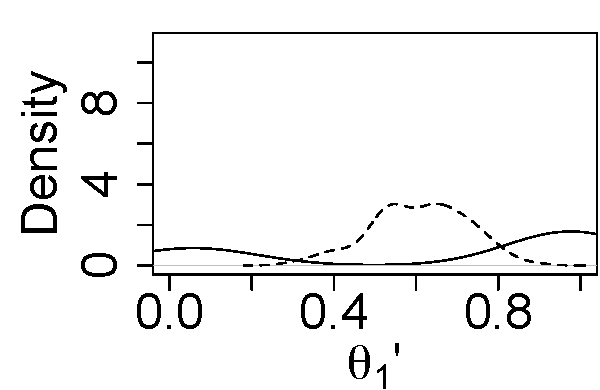
\includegraphics[scale=.3]{sims-R-10-4.pdf}}

  
  \end{tabular}
\end{center}
\caption{{\footnotesize Simulated distribution of binomial ordering preferences for a single expression type with $\mu=0.6$ in a standard 2-Alternative Iterated Learning Model (dotted lines) and one with an explicit regularization bias in data production of $\alpha=1.1$ (solid lines). Note that $\theta'_1=\theta_1$ in the standard model. Regularization depends upon $N$ only in the model with an explicit regularization bias.}}
\label{fig:R11} 
\end{figure}

%\setlength\tabcolsep{1pt}
%\begin{figure}[ht]
%\begin{center}
%  \begin{tabular}{lcc}
% & $\nu = 1$ & $\nu = 10$
%  \\
%  $N=10$ & \pbox[c]{\textwidth}{\includegraphics[scale=.3]{sims-1-1.pdf}}
%  & \pbox[c]{\textwidth}{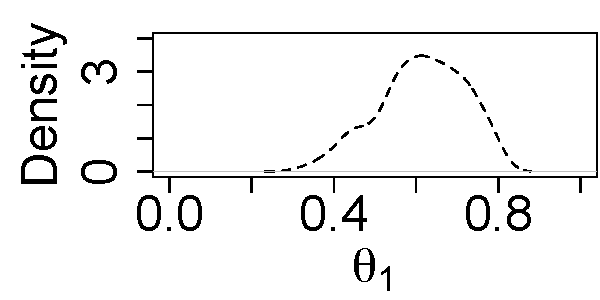
\includegraphics[scale=.3]{sims-10-1.pdf}}
%\\
%  $N=100$ & \pbox[c]{\textwidth}{\includegraphics[scale=.3]{sims-1-2.pdf}}
%  & \pbox[c]{\textwidth}{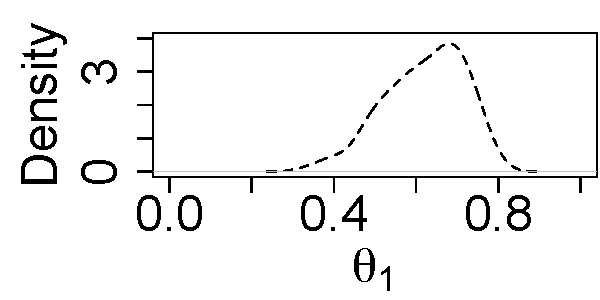
\includegraphics[scale=.3]{sims-10-2.pdf}}
%\\
%  $N=200$ & \pbox[c]{\textwidth}{\includegraphics[scale=.3]{sims-1-3.pdf}}
%  & \pbox[c]{\textwidth}{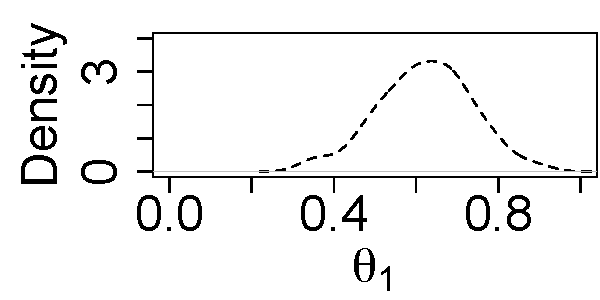
\includegraphics[scale=.3]{sims-10-3.pdf}}
%\\
%  $N=500$ & \pbox[c]{\textwidth}{\includegraphics[scale=.3]{sims-1-4.pdf}}
%  & \pbox[c]{\textwidth}{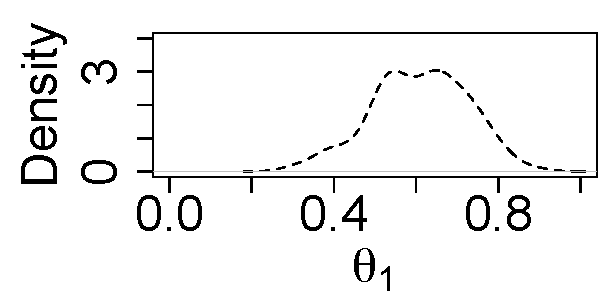
\includegraphics[scale=.3]{sims-10-4.pdf}}
%\\
%
%  
%  \end{tabular}
%\end{center}
%\caption{{\footnotesize Distribution of binomial ordering preferences in a standard 2-Alternative Iterated Learning Model \label{fig:R1}}}
%\end{figure}

\section{Emergence of Frequency-Dependent Regularization in Iterated Learning}
\label{sec:emerg-freq-depend}
%
The standard 2-Alternative Iterated Learning Model does not predict frequency-dependent regularization. We now demonstrate that we can predict frequency-dependent regularization by introducing a frequency-\emph{independent} regularization bias into our model. Under this model, frequency-dependent regularization is an emergent property of the interaction of the frequency-independent regularization bias with the bottleneck effect of cultural transmission.


We augment the learning and transmission process as follows. After hearing data, the learner chooses a hypothesis $\theta_1$ as before, then applies a regularization function to produce a new hypothesis $\theta_1'$, then generates data from $\theta_1'$.

The regularization function is the regularized incomplete beta function (equivalently, the cumulative distribution function of the beta distribution), restricted to be symmetric such that it has a single free parameter $\alpha$:
\begin{equation}
f(x;\alpha) = \frac{\int_0^{x}t^{\alpha-1}(1-t)^{\alpha-1}\,\mathrm{d}t}{\mathrm{B}(\alpha,\alpha)}
\end{equation}
As shown in Fig.\ \ref{fig:R}, the bias parameter $\alpha$ controls strength of regularization. When $\alpha=1$, this is the identity function, i.e.\ no explicit regularization is added. As $\alpha$ increases, the regularization bias grows stronger. 

 \begin{wrapfigure}{L}{0.35\textwidth}
% \begin{figure}[ht]
\begin{center}
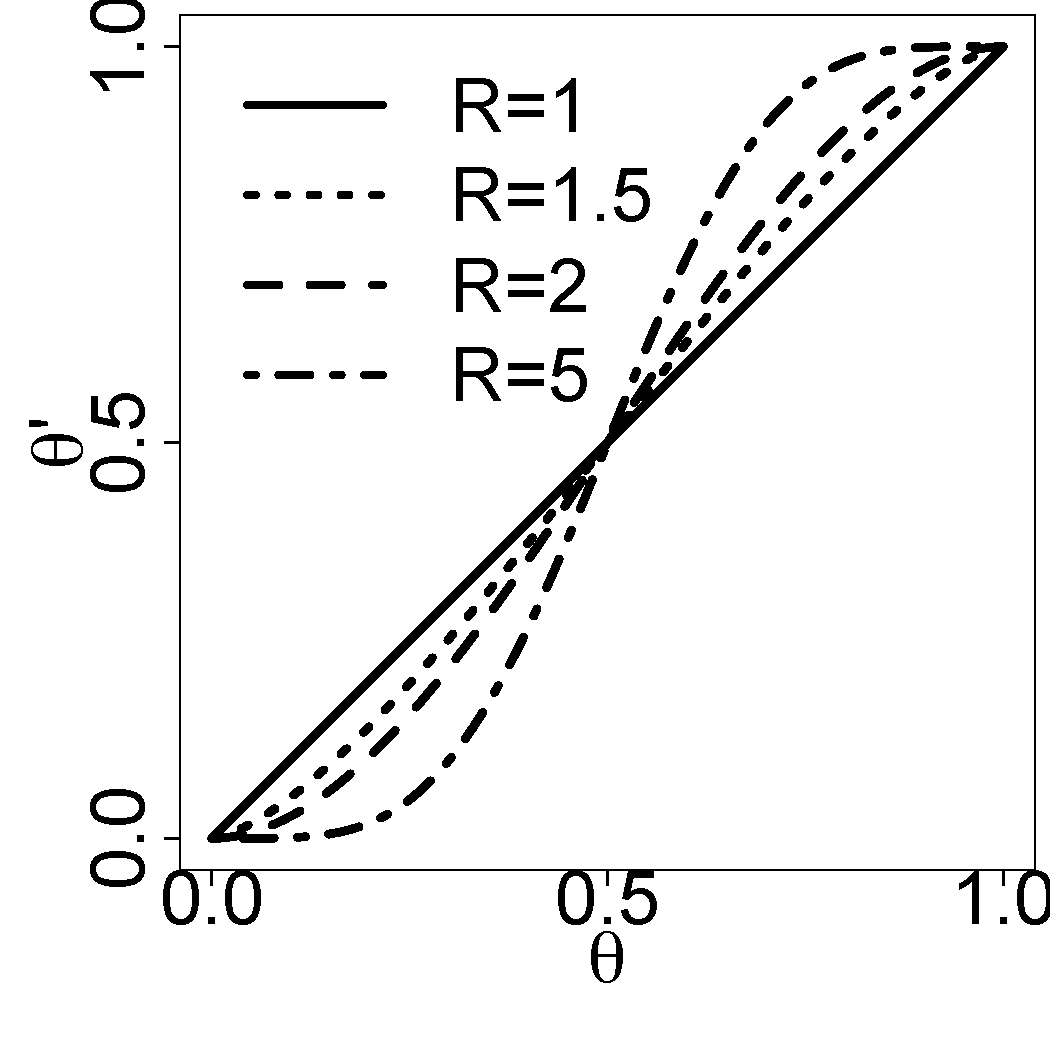
\includegraphics[scale=.2]{R.pdf}
\end{center}
\caption{{\footnotesize Regularization function with different values of $\alpha$ \label{fig:R}}}
\end{wrapfigure}

 \subsection{Results: Frequency-dependent regularization}
 When we repeat the simulations from above using  a non-trivial regularization bias $\alpha=1.1$, we see frequency-dependent regularization in the case with a dense prior (Fig.\ \ref{fig:R11}). Although the regularization bias itself is frequency-independent, frequency-dependence emerges from the interaction of the regularization bias with the process of cultural transmission: At lower frequencies, there is not sufficient data for the regularization bias to overcome the prior. At higher frequencies, the regularization bias becomes increasingly dominant as there is increasingly enough data for the effects of this bias to be carried across generations. Even a relatively weak bias ($\alpha=1.1$) can produce noticeable regularization when compounded across generations. However, the prior always continues to exert some influence; thus, even the highest frequency expressions do not become completely regularized.
 
 Another linguistically accurate property of this model is that for sufficiently high values of $N$, the distribution over hypotheses includes a mode on the opposite side of 0.5 from the prior. Thus the model correctly predicts that at high enough frequencies, an expression can become idiosyncratically preferred in the opposite of its compositionally predicted direction (as in ``ladies and gentlemen'').
 

\subsection{Results: Simulating corpus data}\label{corpus}
Having demonstrated that our augmented model produces frequency-dependent regularization, we now show that it additionally predicts the true language-wide distribution of binomial preference strengths seen in corpus data. The target distribution to be accounted for is shown in Fig.\ \ref{fig:corpus}.


We take the true properties of each binomial expression in the corpus: its compositional preference determines $\mu$ and its overall frequency determines $N$. We scale overall frequency counts based on estimated lifetime exposure to 300 million total words (\citeNP[footnote 10]{Levy:2012bj}). The resulting distribution of values $N$ is shown in Fig.\ \ref{fig:extremity}. For each binomial in the corpus, we approximate the stationary distribution by modeling 10 chains of learners for 200 generations each and take the hypothesis $\theta'_1$ of the final generation of each chain.

% \begin{figure}[ht]
%%\begin{wrapfigure}[14]{L}{0.5\textwidth}
%\begin{center}
%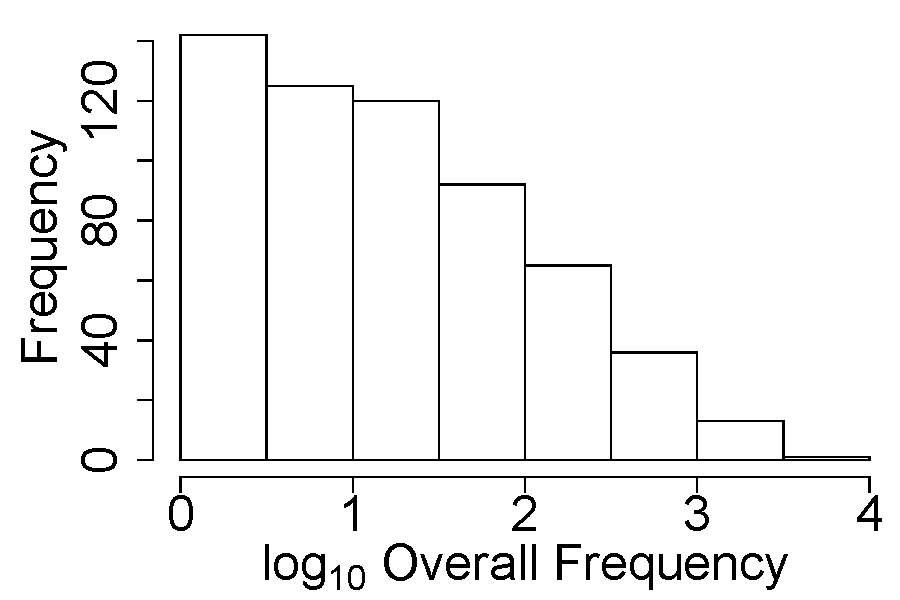
\includegraphics[scale=.25]{N-hist.pdf}
%\end{center}
%\caption{{\footnotesize The distribution over overall frequencies $N$ is non-Zipfian because Morgan and Levy's corpus is restricted to binomial types with at least 1000 occurrences in the Google Books corpus in order to ensure that they have reliable relative frequency estimates. \label{fig:N}}}
%\end{figure}

% \begin{SCfigure}
%\centering
%\caption{{\footnotesize The distribution over overall frequencies $N$ is non-Zipfian because the corpus is restricted to binomial types with at least 1000 occurrences in the Google Books corpus. \label{fig:N}}}
%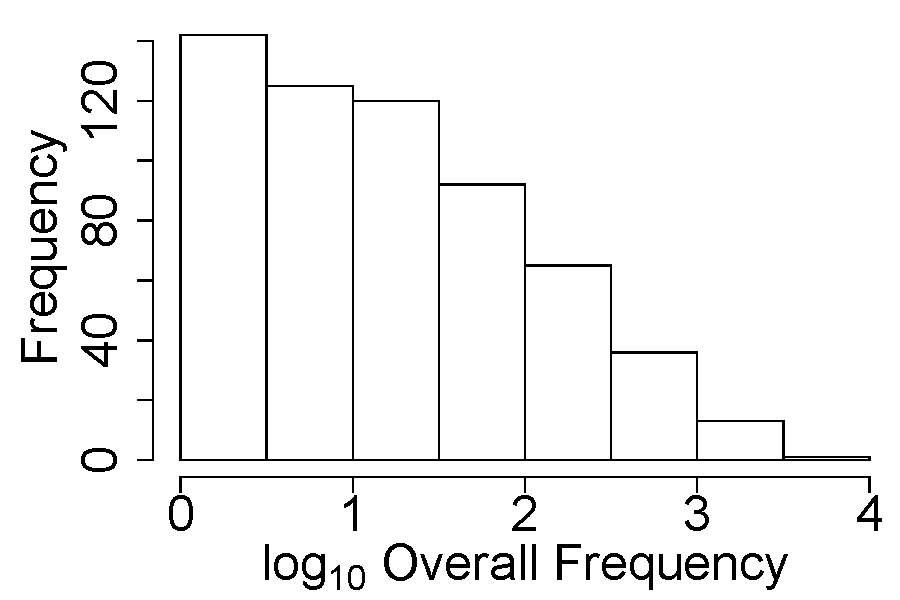
\includegraphics[scale=.25]{N-hist.pdf}
%\end{SCfigure}

Our model has two free parameters, $\nu$ and $\alpha$. We model the corpus data as described above for a range of values of both of these parameters. As shown in Fig.\ \ref{fig:nuxR}, our model displays a trade-off between the prior and the regularization bias as a function of these parameters. At appropriate values, our model correctly predicts the multimodal distribution of corpus data as seen in Fig.\ \ref{fig:corpus}.%\footnote{Why do we predict the \emph{distribution} of binomial expression preferences rather than the preferences for individual binomials? There is stochasticity in how any individual binomial will evolve over time: particularly for high frequency binomials, they can become polarized either in their compositionally preferred direction or non-preferred direction, as shown in Fig ?. We don't expect to be able to predict the individual historical quirks that lead individual items to freeze in one order or another, but we \emph{can} predict the distribution over preferences for items of a given prior $\mu$ with a given frequency $N$. It therefore makes sense for us to test our language-wide predictions against the language-wide distribution rather than testing predictions for any individual item.}


\begin{figure}[t]
\setlength\tabcolsep{1pt}
\begin{center}
%  \begin{tabular}{lccc}
% & $\nu = 10$ & $\nu = 15$ & $\nu = 20$
%  \\
%  $\alpha=1$ & \pbox[c]{\textwidth}{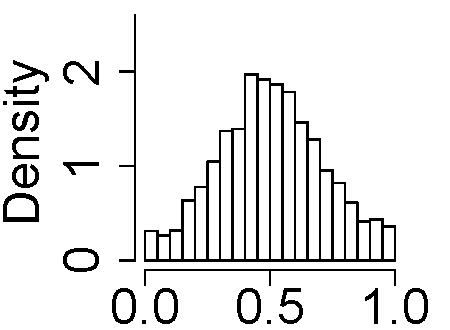
\includegraphics[scale=.3]{nu1R0.pdf}}
%  & \pbox[c]{\textwidth}{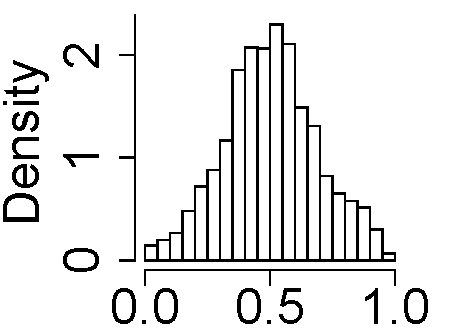
\includegraphics[scale=.3]{nu2R0.pdf}}
%  & \pbox[c]{\textwidth}{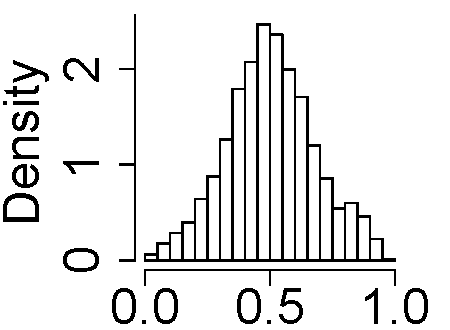
\includegraphics[scale=.3]{nu3R0.pdf}}
%
%  \\
%  $\alpha=1.1$ & \pbox[c]{\textwidth}{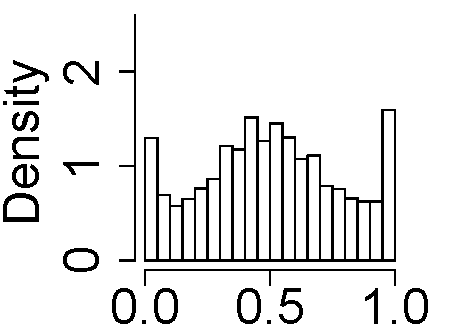
\includegraphics[scale=.3]{nu1R1.pdf}}
%  & \pbox[c]{\textwidth}{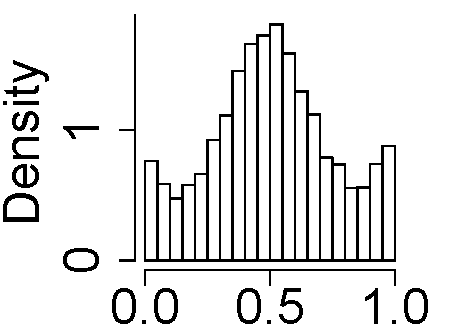
\includegraphics[scale=.3]{nu2R1.pdf}}
%  & \pbox[c]{\textwidth}{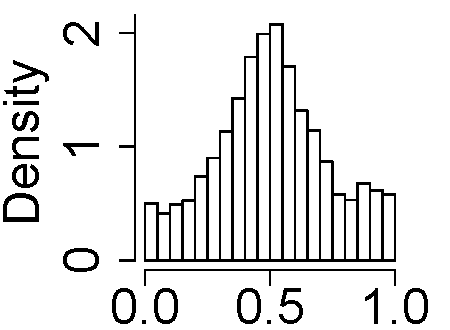
\includegraphics[scale=.3]{nu3R1.pdf}}
%%  & \pbox[c]{\textwidth}{\includegraphics[scale=.3]{nu4R1.pdf}}
%
%  
%  \\
%  $\alpha=1.3$ & \pbox[c]{\textwidth}{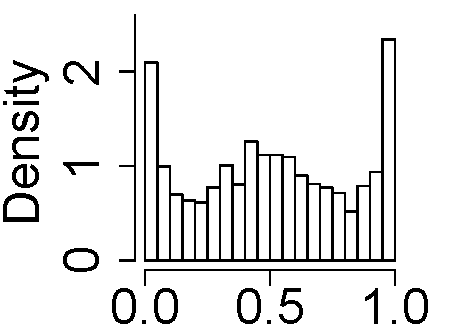
\includegraphics[scale=.3]{nu1R2.pdf}}
%  & \pbox[c]{\textwidth}{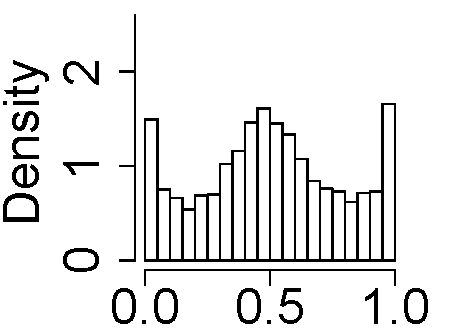
\includegraphics[scale=.3]{nu2R2.pdf}}
%  & \pbox[c]{\textwidth}{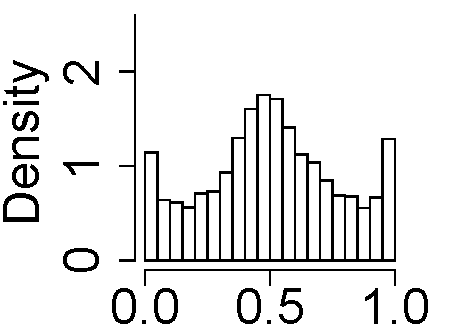
\includegraphics[scale=.3]{nu3R2.pdf}}
%%  & \pbox[c]{\textwidth}{\includegraphics[scale=.3]{nu4R2.pdf}}
%
%  \\
%  $\alpha=1.5$ & \pbox[c]{\textwidth}{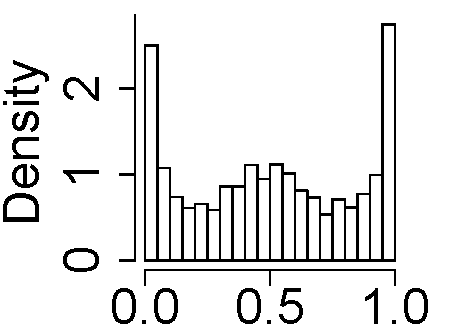
\includegraphics[scale=.3]{nu1R3.pdf}}
%  & \pbox[c]{\textwidth}{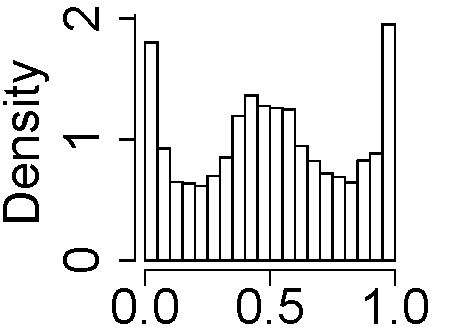
\includegraphics[scale=.3]{nu2R3.pdf}}
%  & \pbox[c]{\textwidth}{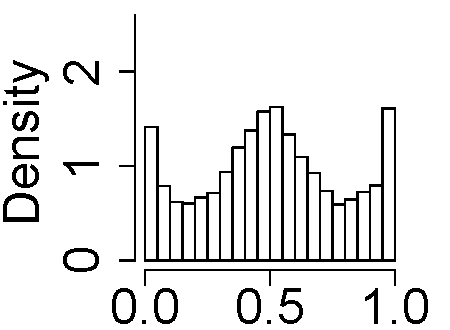
\includegraphics[scale=.3]{nu3R3.pdf}}
%%  & \pbox[c]{\textwidth}{\includegraphics[scale=.3]{nu4R3.pdf}}
%
%
%  
%  \end{tabular}
  
    \begin{tabular}{lcccc}
    & $\alpha=1$ & $\alpha=1.1$ & $\alpha=1.3$ & $\alpha=1.5$
  \\
  $\nu=10$ & \pbox[c]{\textwidth}{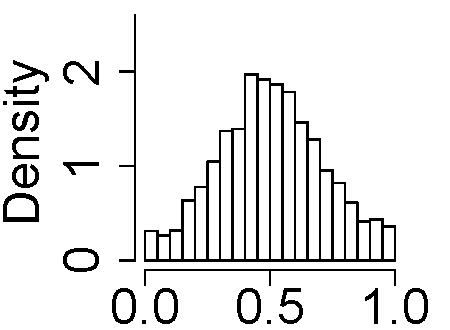
\includegraphics[scale=.25]{nu1R0.pdf}} &
\pbox[c]{\textwidth}{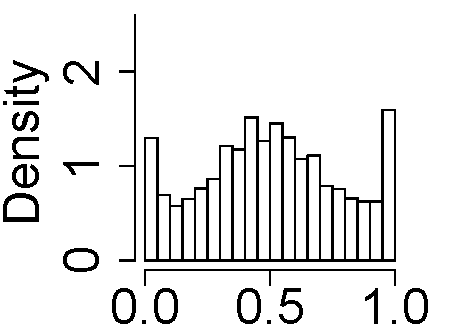
\includegraphics[scale=.25]{nu1R1.pdf}} &
\pbox[c]{\textwidth}{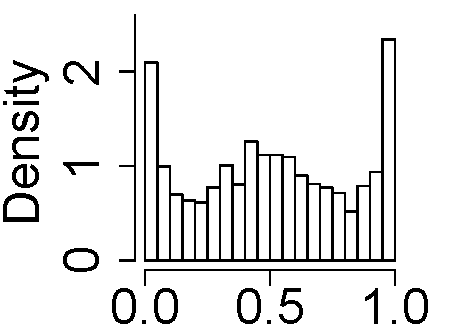
\includegraphics[scale=.25]{nu1R2.pdf}} &
\pbox[c]{\textwidth}{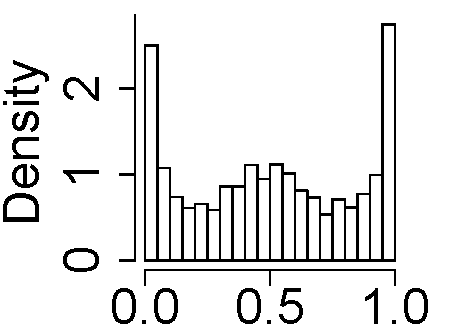
\includegraphics[scale=.25]{nu1R3.pdf}}

  \\
  $\nu=15$ & \pbox[c]{\textwidth}{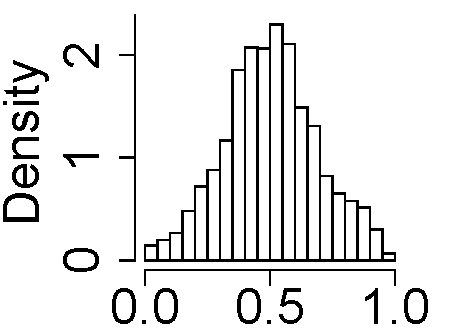
\includegraphics[scale=.25]{nu2R0.pdf}} &
\pbox[c]{\textwidth}{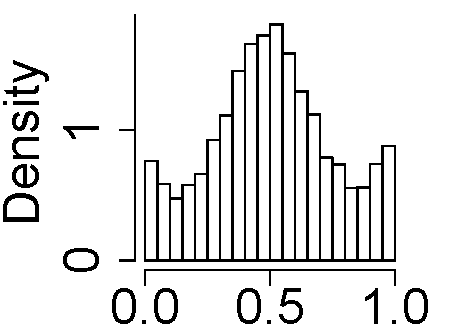
\includegraphics[scale=.25]{nu2R1.pdf}} &
\pbox[c]{\textwidth}{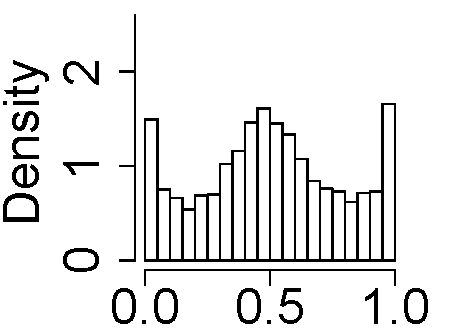
\includegraphics[scale=.25]{nu2R2.pdf}} &
\pbox[c]{\textwidth}{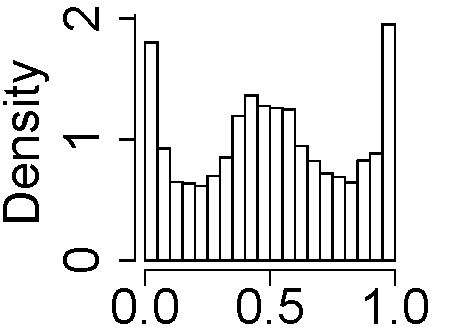
\includegraphics[scale=.25]{nu2R3.pdf}}

  \\
  $\nu=20$ & \pbox[c]{\textwidth}{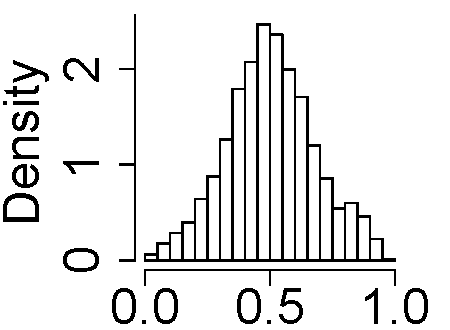
\includegraphics[scale=.25]{nu3R0.pdf}} &
\pbox[c]{\textwidth}{\includegraphics[scale=.25]{nu3R1.pdf}} &
\pbox[c]{\textwidth}{\includegraphics[scale=.25]{nu3R2.pdf}} &
\pbox[c]{\textwidth}{\includegraphics[scale=.25]{nu3R3.pdf}}


  
  \end{tabular}
  
\end{center}
\caption{{\footnotesize Predicted distribution of $\theta'_1$. We see a trade-off between effects of the prior and the regularization bias. When the prior is stronger (high $\nu$, low $\alpha$), we see a unimodal distribution of preferences, similar to Fig.\ \ref{fig:logistic}. When the regularization bias is stronger (low $\nu$, high $\alpha$), we see too much regularization. At appropriate values of $\alpha$ and $\nu$, we see the correct multimodal distribution of preferences as seen in corpus data (Fig.\ \ref{fig:corpus}).  \label{fig:nuxR}}}
\end{figure}




\section{Conclusion}
\label{sec:conclusion}
%
We have demonstrated that a frequency-independent regularization bias in data generation, combined with cultural transmission, can produce the pattern of frequency-dependent regularization of binomial ordering preferences seen in corpus data. Cultural transmission creates frequency-dependence by introducing a bottleneck effect that favors prior knowledge at lower frequencies while allowing the regularization bias to be increasingly well transmitted at higher frequencies. This finding sheds light on the origins of linguistic structure in two important ways: one, it confirms earlier demonstrations of a bias to regularize when learning stochastic linguistic items. Second, it shows that this bias can apply equally across all levels of frequency, but that the distribution of idiosyncrasy seen in the language emerges from the interaction of individuals' cognitive biases with the bottleneck effect of cultural transmission. Additionally, we have expanded the empirical coverage of iterated-learning models, showing that they can account not only for qualitative generalizations in natural language and data from laboratory experiments, but also detailed patterns of naturalistic corpus data.  As we hope to have shown, binomial ordering preferences are a particularly suitable test case for iterated learning models, at once theoretically interesting, data-rich, and computationally tractable.

%\begin{figure}[ht]
%\begin{center}
%  \begin{tabular}{lcccc}
%%  & \multicolumn{4}{c|}{MAP} & \multicolumn{4}{c}{Sampling} \\ \hline
%  & $\nu = 1$ & $\nu = 5$ & $\nu = 10$ & $\nu = 20$
%  \\
%  $R=1.2$ & \pbox[c]{\textwidth}{\includegraphics[scale=.25]{sampling_nu1R1.pdf}}
%  & \pbox[c]{\textwidth}{\includegraphics[scale=.25]{sampling_nu2R1.pdf}}
%  & \pbox[c]{\textwidth}{\includegraphics[scale=.25]{sampling_nu3R1.pdf}}
%  & \pbox[c]{\textwidth}{\includegraphics[scale=.25]{sampling_nu4R1.pdf}}
%
%  
%  \\
%  $R=1.6$ & \pbox[c]{\textwidth}{\includegraphics[scale=.25]{sampling_nu1R2.pdf}}
%  & \pbox[c]{\textwidth}{\includegraphics[scale=.25]{sampling_nu2R2.pdf}}
%  & \pbox[c]{\textwidth}{\includegraphics[scale=.25]{sampling_nu3R2.pdf}}
%  & \pbox[c]{\textwidth}{\includegraphics[scale=.25]{sampling_nu4R2.pdf}}
%
%  \\
%  $R=2.0$ & \pbox[c]{\textwidth}{\includegraphics[scale=.25]{sampling_nu1R3.pdf}}
%  & \pbox[c]{\textwidth}{\includegraphics[scale=.25]{sampling_nu2R3.pdf}}
%  & \pbox[c]{\textwidth}{\includegraphics[scale=.25]{sampling_nu3R3.pdf}}
%  & \pbox[c]{\textwidth}{\includegraphics[scale=.25]{sampling_nu4R3.pdf}}
%
%
%  
%  \end{tabular}
%\end{center}
%\caption{{\footnotesize An example graph.  All labels are legible, and
%    this caption is in $\backslash$footnotesize. \label{fig:sampling}}}
%\end{figure}

%
\section*{Acknowledgements}

[Acknowledgments withheld in submitted version to maintain author anonymity during review]
%\vspace{1cm}
% We gratefully acknowledge support from research grants NSF 0953870 and NICHD R01HD065829 and fellowships from the Alfred P. Sloan Foundation and the Center for Advanced Study in the Behavioral Sciences to Roger Levy.


\bibliographystyle{apacite}
\bibliography{evolang11} 

\end{document}
